\documentclass{article}
\usepackage{../style/latex/dhruv_theory_style}

% -------------------------------------------------------
% Document metadata
% -------------------------------------------------------
\title{\textbf{DSC 190/291 --- Assignment 2}}
\author{Dhruv Patel}
\date{\today}
 
% =======================================================
\begin{document}
% =======================================================
 
\maketitle
\tableofcontents
\newpage
 
% =======================================================
\section{Part A: Unions of Two Intervals on the Line}
% =======================================================
 
\subsection{A.1 --- Restriction Patterns}
 
\begin{summarybox}
\textbf{Claim.} A binary labeling $(y_1,\dots,y_n)\in\{0,1\}^n$ of the ordered
points $x_1<\cdots<x_n$ is realizable by $\mathcal{H}_2$ if and only if it
contains \textbf{at most two contiguous ``1-blocks''} (maximal runs of
consecutive 1s).
\end{summarybox}
 
\begin{definition}
A \emph{1-block} in a binary string is a maximal contiguous run of 1s.
The string $0,1,1,0,1,0$ has exactly two 1-blocks: $\{2,3\}$ and $\{5\}$.
\end{definition}
 
\begin{proof}
$(\Rightarrow)$
Suppose $h=\mathbf{1}[x\in I_1\cup I_2]$ for intervals $I_1,I_2\subseteq\R$.
Since $I_j$ is an interval and the sample points are totally ordered, the
set $\{i:x_i\in I_j\}$ is a contiguous run of indices (possibly empty).
Hence $h$ restricted to the sample produces at most two contiguous 1-blocks.
 
$(\Leftarrow)$
Suppose the labeling has at most two 1-blocks.
\begin{itemize}
  \item \textbf{Zero 1-blocks:} Take $I_1=I_2=\emptyset$.
  \item \textbf{One 1-block} $[x_{i_1},x_{i_2}]$: Take
        $I_1=[x_{i_1},x_{i_2}]$, $I_2=\emptyset$.
  \item \textbf{Two 1-blocks} $[x_{i_1},x_{i_2}]$ and $[x_{j_1},x_{j_2}]$
        with $i_2<j_1$: Take $I_1=[x_{i_1},x_{i_2}]$, $I_2=[x_{j_1},x_{j_2}]$.
\end{itemize}
In all cases the labeling is realized exactly.
\end{proof}
 
\begin{remark}
Any labeling with three or more separate 1-blocks requires three disjoint
intervals, which is impossible for a union of only two.
\end{remark}
 
% -------------------------------------------------------
\subsection{A.2 --- Exact Growth Function}
% -------------------------------------------------------
 
\begin{summarybox}
\textbf{Theorem.}
\[
  \Gamma_{\mathcal{H}_2}(n)
  \;=\;
  \binom{n+1}{0}+\binom{n+1}{2}+\binom{n+1}{4}.
\]
\end{summarybox}
 
\subsubsection{Slot–Gap Bijection}
 
Label the $n+1$ \emph{gaps} $g_0,g_1,\dots,g_n$, where $g_0$ is before $x_1$,
$g_k$ is between $x_k$ and $x_{k+1}$ for $k=1,\dots,n-1$, and $g_n$ is after
$x_n$.
 
A 1-block spanning $[x_i,x_j]$ corresponds to \emph{entering} at gap $g_{i-1}$
and \emph{exiting} at gap $g_j$. Two 1-blocks select four gaps
$s_1<s_2<s_3<s_4$: block one runs from $x_{s_1+1}$ to $x_{s_2}$, block two
from $x_{s_3+1}$ to $x_{s_4}$. Because $s_2<s_3$, the point
$x_{s_2+1}$ lies strictly between the two blocks and is labeled 0, so the two
blocks are always genuinely separated.
 
\begin{proof}[Proof of Theorem]
Count by number of 1-blocks $m\in\{0,1,2\}$.
\begin{itemize}
  \item $m=0$: choose 0 gaps from the $n+1$ available:
        $\binom{n+1}{0}=1$.
  \item $m=1$: choose 2 gaps $s_1<s_2$ from $\{0,\dots,n\}$:
        $\binom{n+1}{2}$.
  \item $m=2$: choose 4 gaps $s_1<s_2<s_3<s_4$ from $\{0,\dots,n\}$:
        $\binom{n+1}{4}$.
\end{itemize}
These cases are disjoint and exhaustive, so
\[
  \Gamma_{\mathcal{H}_2}(n)=\binom{n+1}{0}+\binom{n+1}{2}+\binom{n+1}{4}.
\]
\end{proof}
 
\subsubsection{Small-Case Verification}
 
\begin{center}
\begin{tabular}{cccc}
\toprule
$n$ & Formula & $2^n$ & Realizable? \\
\midrule
1 & $1+1+0=2$ & 2 & all \\
2 & $1+3+0=4$ & 4 & all \\
3 & $1+6+1=8$ & 8 & all \\
4 & $1+10+5=16$ & 16 & all \\
5 & $1+15+15=31$ & 32 & one missing ($10101$) \\
\bottomrule
\end{tabular}
\end{center}
 
% -------------------------------------------------------
\subsection{A.3 --- VC Dimension and Mistake Bound}
% -------------------------------------------------------
 
\begin{summarybox}
$\operatorname{VCdim}(\mathcal{H}_2)=4$.
\end{summarybox}
 
\begin{proof}
\textbf{Lower bound ($\ge4$).}
We show any 4 ordered points are shattered.
From the table above, $\Gamma_{\mathcal{H}_2}(4)=16=2^4$, so all 16
labelings of 4 points are realizable.
 
\textbf{Upper bound ($\le5$).}
For any 5 ordered points, the alternating labeling $1,0,1,0,1$ has three
1-blocks and is not realizable by $\mathcal{H}_2$. Hence no 5 points are
shattered.
\end{proof}
 
\subsubsection{Halving Mistake Bound}
 
In the realizable online transductive setting on a pool of $n$ points, the
Halving algorithm makes at most
\[
  M \;\le\; \log_2 \Gamma_{\mathcal{H}_2}(n)
    \;=\; \log_2\!\left[\binom{n+1}{0}+\binom{n+1}{2}+\binom{n+1}{4}\right]
\]
mistakes.
 
\subsubsection{Comparison with Sauer--Shelah}
 
The Sauer--Shelah bound with $d=\operatorname{VCdim}(\mathcal{H}_2)=4$ gives
\[
  \Gamma_{\mathcal{H}_2}(n)\;\le\;\sum_{k=0}^{4}\binom{n}{k}.
\]
Applying Pascal's identity $\binom{n+1}{k}=\binom{n}{k}+\binom{n}{k-1}$:
\[
  \binom{n+1}{2}=\binom{n}{2}+n,
  \qquad
  \binom{n+1}{4}=\binom{n}{4}+\binom{n}{3}.
\]
Therefore
\[
  \binom{n+1}{0}+\binom{n+1}{2}+\binom{n+1}{4}
  =1+n+\binom{n}{2}+\binom{n}{3}+\binom{n}{4}
  =\sum_{k=0}^{4}\binom{n}{k}.
\]
\textbf{The two quantities are equal.}
This means $\mathcal{H}_2$ is a \emph{tight} example for Sauer--Shelah: the
class achieves the maximum possible number of dichotomies at every sample size.
Such tightness occurs when, for every subset $S$, the restriction $\mathcal{H}_2|_S$
is as rich as possible given the VC dimension — equivalently, the class
shatters every subset of size $d$ (a property sometimes called \emph{maximum
classes}).
 
% -------------------------------------------------------
\subsection{A.4 --- Tightness of Sauer--Shelah}
% -------------------------------------------------------
 
\begin{summarybox}
\textbf{Construction.}
For integers $n\ge d\ge 0$, let $\mathcal{X}=\R$ and
\[
  \mathcal{H}^{(2p)}
  \;=\;
  \Bigl\{
    x\mapsto\mathbf{1}\bigl[x\in\textstyle\bigcup_{j=1}^{p}I_j\bigr]
    :I_1,\dots,I_p\subseteq\R\text{ intervals}
  \Bigr\},
  \quad d=2p.
\]
Then $\operatorname{VCdim}(\mathcal{H}^{(2p)})=2p$ and
$\Gamma_{\mathcal{H}^{(2p)}}(n)=\sum_{k=0}^{2p}\binom{n}{k}$.
\end{summarybox}
 
By the same slot-gap argument generalized to $p$ intervals:
\[
  \Gamma_{\mathcal{H}^{(2p)}}(n)
  =\sum_{m=0}^{p}\binom{n+1}{2m},
\]
which equals $\sum_{k=0}^{2p}\binom{n}{k}$ by repeated Pascal expansion.
The VC dimension is $2p$ because $2p$ points can always be shattered (any
labeling has $\le p$ 1-blocks among $2p$ points where a third block would
need $\ge2p+1$ positions), but the alternating labeling on $2p+1$ points
requires $p+1$ blocks.
 
\textbf{Significance.} The Sauer--Shelah bound is \emph{sharp in the worst
case}: for every $d$, there is a class achieving equality for all $n\ge d$.
No improvement to the bound is possible that depends only on VC dimension.
 
% -------------------------------------------------------
\subsection{A.5 --- AI Proof Audit}
% -------------------------------------------------------
 
\begin{notebox}
\textbf{AI's claim.}
``\ldots one just chooses up to four switch locations among the $n$ sample
positions.  Therefore $\Gamma_{\mathcal{H}_2}(n)=\sum_{j=0}^{4}\binom{n}{j}$.''
\end{notebox}
 
\subsubsection{What Is Incorrect}
 
\textbf{Flaw 1 --- Wrong counting universe.}
A sign change is an event \emph{between} consecutive sample points, not
\emph{at} a sample point.  With $n$ ordered points there are $n+1$ transition
zones (gaps), not $n$.  Choosing $j$ switch locations from $n$ sample
positions gives $\binom{n}{j}$, but the correct count requires
$\binom{n+1}{j}$.
 
\textbf{Flaw 2 --- Parity constraint ignored.}
The argument suggests choosing \emph{any} number of switches from 0 to 4.
However, the formula $\sum_{j=0}^{4}\binom{n}{j}$ includes terms with $j=1$
and $j=3$.  Blocks of 1s at the boundary (e.g.\ $1,1,0,0$) do produce an odd
number of sign changes in the string, but only because the opening boundary
transition is not counted in the AI's scheme.  The AI never justifies why odd
and even counts are treated uniformly, nor why the count from $n$ gaps is
correct.
 
\textbf{Flaw 3 --- Numerically correct but derivation is wrong.}
The AI's final formula $\sum_{j=0}^{4}\binom{n}{j}$ \emph{happens} to equal
the true growth function (as we verified by Pascal's identity), but the
argument does not establish this.  A derivation that arrives at the right
answer by the wrong route is still a flawed proof.
 
\subsubsection{Correct Statement}
 
\begin{theorem}
The growth function of $\mathcal{H}_2$ is
\[
  \Gamma_{\mathcal{H}_2}(n)
  \;=\;
  \binom{n+1}{0}+\binom{n+1}{2}+\binom{n+1}{4}
  \;=\;
  \sum_{k=0}^{4}\binom{n}{k}.
\]
A labeling is realizable iff it has at most two contiguous 1-blocks.
The correct combinatorial argument selects $2m$ boundary gaps from the
$n+1$ available gaps (not sample points) to encode $m$ 1-blocks, giving
$\binom{n+1}{2m}$ labelings with exactly $m$ blocks.
\end{theorem}
 
% =======================================================
\section{Part B: Quadratic Threshold Functions on the Line}
% =======================================================
 
\subsection{B.1 --- A General Upper-Bound Trick}
 
\begin{theorem}
\label{thm:upper-bound-trick}
If there exist $D\ge1$ and $\varphi:\mathcal{X}\to\R^D$ such that every
$h\in\mathcal{H}$ can be written $h(x)=\mathbf{1}[\langle w,\varphi(x)\rangle\ge0]$
for some $w\in\R^D$, then $\operatorname{VCdim}(\mathcal{H})\le D$.
\end{theorem}
 
\begin{proof}
Let $\mathcal{H}_{\mathrm{hs}}=\{x\mapsto\mathbf{1}[\langle w,x\rangle\ge0]:w\in\R^D\}$
be the class of homogeneous halfspaces on $\R^D$.
For any sample $S=\{x_1,\dots,x_n\}\subseteq\mathcal{X}$, every dichotomy
that $\mathcal{H}$ induces on $S$ is also induced by $\mathcal{H}_{\mathrm{hs}}$
on the mapped sample $\varphi(S)=\{\varphi(x_1),\dots,\varphi(x_n)\}$:
\[
  |\mathcal{H}(S)| \;\le\; |\mathcal{H}_{\mathrm{hs}}(\varphi(S))|.
\]
By the Week-2 result, $\operatorname{VCdim}(\mathcal{H}_{\mathrm{hs}})=D$.
Sauer--Shelah then gives $|\mathcal{H}_{\mathrm{hs}}(\varphi(S))|<2^n$ for
all $n>D$.
Therefore $|\mathcal{H}(S)|<2^n$ for all $n>D$, so $\mathcal{H}$ cannot
shatter any set of size $>D$.
Hence $\operatorname{VCdim}(\mathcal{H})\le D$.
\end{proof}
 
% -------------------------------------------------------
\subsection{B.2 --- Applying the Trick to Quadratic Thresholds}
% -------------------------------------------------------
 
\begin{summarybox}
\textbf{Feature map.}
\[
  \varphi:\R\to\R^3,
  \qquad
  \varphi(x)=(x^2,\,x,\,1).
\]
\end{summarybox}
 
\begin{proof}[Proof that the map works]
Every $h\in\mathcal{H}_{\mathrm{quad}}$ has the form $h(x)=\mathbf{1}[ax^2+bx+c\ge0]$
for $(a,b,c)\ne(0,0,0)$.  Setting $w=(a,b,c)\in\R^3$,
\[
  \langle w,\varphi(x)\rangle
  =a\cdot x^2+b\cdot x+c\cdot 1
  =ax^2+bx+c,
\]
so $h(x)=\mathbf{1}[\langle w,\varphi(x)\rangle\ge0]$.
\end{proof}
 
By Theorem~\ref{thm:upper-bound-trick} with $D=3$,
\[
  \operatorname{VCdim}(\mathcal{H}_{\mathrm{quad}})\;\le\;3.
\]
 
% -------------------------------------------------------
\subsection{B.3 --- Exact Restriction Patterns}
% -------------------------------------------------------
 
\begin{summarybox}
\textbf{Characterization.}
A labeling $(y_1,\dots,y_n)$ is realizable by $\mathcal{H}_{\mathrm{quad}}$
iff it falls into one of the following two types:
\begin{description}
  \item[Type A (at most one 1-block):] the 1-labeled positions form a
    single contiguous run (including empty or the full sequence).
  \item[Type B (prefix-suffix):] $y_1=1$ and $y_n=1$, and there is a
    contiguous interior block of 0s separating two 1-blocks.
    Formally: $\exists\,1\le i<j\le n-1$ such that
    $y_1=\cdots=y_i=1$, $y_{i+1}=\cdots=y_j=0$, $y_{j+1}=\cdots=y_n=1$.
\end{description}
All other labelings are \emph{not} realizable.
\end{summarybox}
 
\begin{proof}
The set $\{x:ax^2+bx+c\ge0\}$ takes exactly the following shapes:
 
\medskip
\begin{center}
\begin{tabular}{lll}
\toprule
Case & Shape of nonneg.\ region & On sample \\
\midrule
$a<0$, $\Delta>0$ & closed interval $[r_1,r_2]$ & one 1-block (Type A) \\
$a<0$, $\Delta\le0$ & empty or single point & 0 or trivial 1-block (Type A) \\
$a>0$, $\Delta>0$ & $(-\infty,r_1]\cup[r_2,\infty)$ & prefix 1s + suffix 1s (Type B) \\
$a>0$, $\Delta\le0$ & all of $\R$ or single point & all 1s or one point (Type A) \\
$a=0$, $b\ne0$ & halfline & prefix or suffix of 1s (Type A) \\
$a=b=0$ & all $\R$ or $\emptyset$ & all 1s or all 0s (Type A) \\
\bottomrule
\end{tabular}
\end{center}
\medskip
 
Here $\Delta=b^2-4ac$ is the discriminant.
Type~A covers all cases with $a\le0$ or $a>0,\Delta\le0$.
Type~B arises exactly when $a>0$ and $\Delta>0$, giving the
complement-of-interval pattern which on the sample becomes a prefix of 1s
followed by an interior 0-block followed by a suffix of 1s.
No other 1-block pattern is achievable, ruling out, for example,
the labeling $0,1,0,1,0$.
\end{proof}
 
% -------------------------------------------------------
\subsection{B.4 --- Exact Growth Function and VC Dimension}
% -------------------------------------------------------
 
\begin{theorem}
\[
  \Gamma_{\mathcal{H}_{\mathrm{quad}}}(n)
  \;=\;
  n^2-n+2.
\]
\end{theorem}
 
\begin{proof}
Count realizable labelings by type.
 
\textbf{Type A (at most one 1-block).}
The number of contiguous 1-blocks in a string of length $n$ is
$\binom{n+1}{2}$ (one for each pair of gap positions bounding the block),
plus 1 for the all-zeros labeling:
\[
  |\text{Type A}| = 1+\binom{n+1}{2} = 1+\frac{n(n+1)}{2}.
\]
 
\textbf{Type B (prefix-suffix).}
Choose prefix length $a\ge1$, interior 0-block length $b\ge1$, suffix length
$c=n-a-b\ge1$.  The number of valid $(a,b)$ pairs with $a\ge1$, $b\ge1$,
$a+b\le n-1$ is, by substitution $a'=a-1\ge0$, $b'=b-1\ge0$,
$c'=n-1-a-b\ge0$ with $a'+b'+c'=n-3$:
\[
  |\text{Type B}| = \binom{n-1}{2} = \frac{(n-1)(n-2)}{2}.
\]
 
\textbf{Total.}
\[
  \Gamma_{\mathcal{H}_{\mathrm{quad}}}(n)
  = 1+\frac{n(n+1)}{2}+\frac{(n-1)(n-2)}{2}
  = 1+\frac{n^2+n+n^2-3n+2}{2}
  = 1+\frac{2n^2-2n+2}{2}
  = n^2-n+2.
\]
\end{proof}
 
\subsubsection{Small-Case Verification}
 
\begin{center}
\begin{tabular}{cccc}
\toprule
$n$ & $n^2-n+2$ & $2^n$ & Non-realizable \\
\midrule
1 & 2 & 2 & 0 \\
2 & 4 & 4 & 0 \\
3 & 8 & 8 & 0 \\
4 & 14 & 16 & 2 (viz.\ $0101$, $1010$) \\
5 & 22 & 32 & 10 \\
\bottomrule
\end{tabular}
\end{center}
 
\subsubsection{Exact VC Dimension}
 
\begin{summarybox}
$\operatorname{VCdim}(\mathcal{H}_{\mathrm{quad}})=3$.
\end{summarybox}
 
\begin{proof}
$\Gamma_{\mathcal{H}_{\mathrm{quad}}}(3)=8=2^3$ (all 8 labelings of 3
points are realizable), so 3 points are shattered.
$\Gamma_{\mathcal{H}_{\mathrm{quad}}}(4)=14<16=2^4$, so no 4 points are
shattered.
Explicitly: for any $x_1<x_2<x_3<x_4$, the labeling $0,1,0,1$ has two
non-boundary 1-blocks and is not realizable.
Hence $\operatorname{VCdim}(\mathcal{H}_{\mathrm{quad}})=3$,
consistent with the upper bound $\le3$ from Theorem~\ref{thm:upper-bound-trick}.
\end{proof}
 
\subsubsection{Comparison with Sauer--Shelah}
 
With $d=3$, the Sauer--Shelah bound gives
\[
  \sum_{k=0}^{3}\binom{n}{k}
  = 1+n+\frac{n(n-1)}{2}+\frac{n(n-1)(n-2)}{6}
  = \Theta(n^3).
\]
Our exact formula $n^2-n+2=\Theta(n^2)$ is \textbf{strictly smaller}.
The VC-based bound is not tight here.
 
\textbf{What this says.}
VC dimension controls only the \emph{degree} of the polynomial bounding
the growth function, not the coefficient or lower-order terms.
$\mathcal{H}_{\mathrm{quad}}$ has VC dimension 3 yet grows like $n^2$, while a
generic VC-3 class can grow like $n^3/6$.
The algebraic constraint (the nonneg region of a quadratic has
topologically restricted shape) makes $\mathcal{H}_{\mathrm{quad}}$ much
leaner than a ``generic'' class of the same VC dimension.
VC dimension alone is therefore a coarse summary of finite-pool richness.
 
% -------------------------------------------------------
\subsection{B.5 --- AI Proof Audit}
% -------------------------------------------------------
 
\begin{notebox}
\textbf{AI's claim.}
``\ldots one chooses up to two change-points among the $n-1$ gaps and
gets $\Gamma_{\mathcal{H}_{\mathrm{quad}}}(n)=\sum_{j=0}^{2}\binom{n-1}{j}$.
In particular, $\operatorname{VCdim}(\mathcal{H}_{\mathrm{quad}})=3$.''
\end{notebox}
 
\subsubsection{What Is Incorrect}
 
\textbf{Flaw 1 --- Ignores the $a>0$ (upward-parabola) case.}
The AI considers only labelings produced by a single bounded interval
(arising from $a<0$). The case $a>0$ yields the complement of a bounded
interval: a prefix of 1s, an interior 0-block, and a suffix of 1s.
This pattern also has at most 2 sign changes but is not captured by the
``choose a change-point'' scheme the AI describes.
 
\textbf{Flaw 2 --- Wrong counting universe.}
The change-point of a quadratic lies in one of the $n+1$ gaps between
sample points (including boundary gaps before $x_1$ and after $x_n$),
not in one of the $n-1$ interior gaps. A halfline $\{x\ge r\}$ with
$r<x_1$ gives a labeling of all-1s; the sign change is in gap $g_0$,
which the AI's scheme does not count.
 
\textbf{Flaw 3 --- Formula gives wrong values.}
The AI's formula for $n=3$:
\[
  \sum_{j=0}^{2}\binom{2}{j} = 1+2+1 = 4 \ne 8 = 2^3.
\]
But all 8 labelings of 3 points are realizable (verified above), so
the correct value is $8$. The AI's formula gives 4, which would imply
$\operatorname{VCdim}\le2$, contradicting the correct answer of 3.
The conclusion is stated correctly, but it does not follow from the
(incorrect) formula.
 
\subsubsection{Correct Statement}
 
\begin{theorem}
The growth function of $\mathcal{H}_{\mathrm{quad}}$ is
\[
  \Gamma_{\mathcal{H}_{\mathrm{quad}}}(n) = n^2-n+2,
\]
equal to $1+\binom{n+1}{2}+\binom{n-1}{2}$.
A labeling is realizable iff it has at most one contiguous 1-block
(Type A) or is a prefix-suffix pattern (Type B).
The VC dimension is $\operatorname{VCdim}(\mathcal{H}_{\mathrm{quad}})=3$:
three points are shattered (all $2^3=8$ labelings realizable), while four
points cannot be shattered (e.g.\ $0,1,0,1$ is not realizable).
\end{theorem}
 
% =======================================================
\section{Part C: AI Usage Report}
% =======================================================
 
\subsection{Parts Where AI Was Used}
 
\begin{enumerate}
  \item \textbf{Part A:} Formalizing the slot--gap bijection for the growth
    function.  I used AI to help articulate why the counting universe has
    $n+1$ gaps rather than $n$ sample points, and to check whether the
    two-block case (four chosen gaps) is always genuinely separated.
 
  \item \textbf{Part B:} Working through the case analysis of the nonneg
    region of a quadratic ($a>0$ vs.\ $a<0$ vs.\ $a=0$), and algebraically
    simplifying $1+\binom{n+1}{2}+\binom{n-1}{2}$ to $n^2-n+2$.
 
  \item \textbf{Parts A.5 and B.5:} Structuring the AI audit sections.
    I used AI both to generate candidate flawed arguments and then to reason
    about what was wrong with them.
 
  \item \textbf{Lean files and Python script:} AI was used to draft the Lean
    formalization scaffolding (B.1 and B.2) and the enumeration script.
    I verified the Lean types and the script's output against hand calculations.
\end{enumerate}
 
\subsection{Suggestions Accepted}
 
\begin{itemize}
  \item The slot--gap framework: treating the $n+1$ boundary gaps as the
    primary counting objects made the bijection clean and bijective.
    This was cleaner than my initial approach of directly counting pairs
    $(i,j)$ with $i\le j$.
 
  \item The closed-form simplification $n^2-n+2$ for the quadratic growth
    function.  I verified this algebraically and by small cases.
 
  \item Using the discriminant $\Delta=b^2-4ac$ as the organizing criterion
    for the Part B case analysis.
\end{itemize}
 
\subsection{Suggestions Rejected or Modified}
 
\begin{itemize}
  \item An early draft of A.2 stated the formula as $\sum_{j=0}^{4}\binom{n}{j}$
    without deriving it.  I required the slot--gap argument because deriving
    $\binom{n+1}{2k}$ first and then applying Pascal is more transparent than
    directly asserting the Sauer--Shelah form.
 
  \item An early draft of B.3 missed the prefix-suffix (Type B) patterns
    entirely.  I corrected this by explicitly enumerating all shapes of
    $\{ax^2+bx+c\ge0\}$ by the sign of $a$ and the discriminant.
 
  \item The AI initially described Type B patterns as having ``two interior
    1-blocks''; I corrected this to specify that one block must be a prefix
    and the other a suffix, which is the key algebraic constraint.
\end{itemize}
 
\subsection{Verification}
 
\begin{itemize}
  \item \textbf{Small cases:} For $n=1,2,3,4,5$ I explicitly enumerated all
    $2^n$ binary strings and checked which were realizable by $\mathcal{H}_2$
    and $\mathcal{H}_{\mathrm{quad}}$, confirming both formulas.  This was
    also automated in the accompanying Python script
    (\texttt{enumerate\_check.py}).
 
  \item \textbf{Algebra:} The Pascal identity expansion and the stars-and-bars
    count for Type B were verified step by step.
 
  \item \textbf{VC dimension:} Both the shattering witness (explicit
    hypotheses realizing all $2^d$ labelings) and the impossibility witness
    (a specific non-realizable labeling for $d+1$ points) were constructed
    explicitly.
 
  \item \textbf{Lean files:} The Lean formalization of Theorems B.1 and B.2
    (\texttt{B1\_upper\_bound.lean}, \texttt{B2\_quadratic\_map.lean}) was
    type-checked.
\end{itemize}
 
\subsection{AI Workflow Updates}
 
\textbf{Key update 1: Always check small cases before trusting a formula.}
Both AI audit failures were immediately visible at $n=3$ or $n=4$.  I have
added a ``small-case sanity check'' step to my standard proof-writing checklist.
 
\textbf{Key update 2: Distinguish boundary from interior effects.}
Both audit errors arose from failing to account for patterns touching the
sample boundary (halflines, prefix-suffix patterns).  I now explicitly ask
``what happens at the left edge and right edge of the sample?'' when
formulating any counting argument over ordered sequences.
 
\textbf{Key update 3: Formal enumeration as ground truth.}
Running \texttt{code/enumerate\_check.py} gives exact counts for small $n$
that serve as a reference against which closed-form formulas can be validated
before being trusted.  See Appendix~\ref{app:enum} for the full output and
Figure~\ref{fig:growth} for the plot.
 
% =======================================================
\appendix
% =======================================================
 
% =======================================================
\section{Repository Artifact Map}
\label{app:artifacts}
% =======================================================
 
The course repository for this assignment is structured as follows.
 
\begin{center}
\begin{tabular}{lll}
\toprule
Path & File & Role in write-up \\
\midrule
\texttt{hw2/code/} & \texttt{enumerate\_check.py}  & Brute-force verification of $\Gamma_{\mathcal{H}_2}$ and $\Gamma_{\mathcal{H}_{\mathrm{quad}}}$ \\
\texttt{hw2/lean/} & \texttt{B1\_upper\_bound.lean} & Lean~4 formalization of Theorem~B.1 \\
\texttt{hw2/lean/} & \texttt{B2\_quadratic\_map.lean} & Lean~4 formalization of Theorem~B.2 \\
\texttt{hw2/figures/} & \texttt{growth\_functions.pdf} & Figure~\ref{fig:growth} (growth functions line plot) \\
\texttt{hw2/figures/} & \texttt{enumeration\_table.pdf} & Figure~\ref{fig:table} (enumeration results table) \\
\bottomrule
\end{tabular}
\end{center}
 
To reproduce all artifacts from scratch:
\begin{enumerate}
  \item \textbf{Python enumeration:}
    \texttt{python hw2/code/enumerate\_check.py --n 8}\\
    Requires Python~3.9+ with \texttt{scipy} and \texttt{matplotlib}.
    Produces the console table in Appendix~\ref{app:enum} and
    \texttt{hw2/figures/growth\_functions.pdf}.
  \item \textbf{Lean type-checking:}
    \texttt{lake build} from the repository root (requires Lean~4 with
    Mathlib4 installed via \texttt{lake update}).
    Both \texttt{.lean} files import from Mathlib and type-check with
    one honest \texttt{sorry} for the injectivity detail in B.1 and
    one axiom standing in for the Week-2 halfspace VC-dimension result.
\end{enumerate}
 
% =======================================================
\section{Enumeration Output and Growth-Function Plot}
\label{app:enum}
% =======================================================
 
\subsection{Console output of \texttt{enumerate\_check.py}}
 
The script was run with
\texttt{python code/enumerate\_check.py --n 8 --figures-dir ../figures}.
Every row compares the brute-force count against the closed-form formula;
a \checkmark{} indicates equality.
 
\begin{notebox}
\small
\begin{verbatim}
  n    2^n    |H2|   Gamma_H2(n)  H2 ok  SS(n,4)  H2=SS   |Hq|   Gamma_Hq(n)  Hq ok  SS(n,3)
  1      2       2           2      ✓        2        ✓      2           2       ✓        2
  2      4       4           4      ✓        4        ✓      4           4       ✓        4
  3      8       8           8      ✓        8        ✓      8           8       ✓        8
  4     16      16          16      ✓       16        ✓     14          14       ✓       15
  5     32      31          31      ✓       31        ✓     22          22       ✓       26
  6     64      57          57      ✓       57        ✓     32          32       ✓       42
  7    128      99          99      ✓       99        ✓     44          44       ✓       64
  8    256     163         163      ✓      163        ✓     58          58       ✓       93
 
VC dimension verification:
  VCdim(H2)     >= 4  (all 2^n labelings realizable up to n=4)
  VCdim(H_quad) >= 3  (all 2^n labelings realizable up to n=3)
  VCdim(H2)      < 5  (first n where not all labelings realizable: 5)
  VCdim(H_quad)  < 4  (first n where not all labelings realizable: 4)
 
All formulas verified for n = 1 to 8.
H2 growth function equals Sauer-Shelah bound (tight) for all n.
H_quad Sauer-Shelah is NOT tight (first diverges at n=4).
\end{verbatim}
\end{notebox}
 
Key observations from the table:
\begin{itemize}
  \item The column \texttt{H2 ok} is \checkmark{} for all $n$, confirming
    $\Gamma_{\mathcal{H}_2}(n)=\binom{n+1}{0}+\binom{n+1}{2}+\binom{n+1}{4}$.
  \item The column \texttt{H2=SS} is also \checkmark{} for all $n$, confirming
    that $\mathcal{H}_2$ achieves the Sauer--Shelah bound with equality.
  \item The column \texttt{Hq ok} is \checkmark{} for all $n$, confirming
    $\Gamma_{\mathcal{H}_{\mathrm{quad}}}(n)=n^2-n+2$.
  \item For $n\ge4$, $\Gamma_{\mathcal{H}_{\mathrm{quad}}}(n)<\text{SS}(n,3)$
    (e.g.\ $14$ vs.\ $15$ at $n=4$), confirming the bound is not tight.
\end{itemize}
 
\subsection{Enumeration table figure}
 
Figure~\ref{fig:table} is the same data rendered as a saved figure by the
script (\texttt{figures/enumeration\_table.pdf}).  Blue columns correspond
to $\mathcal{H}_2$; green columns to $\mathcal{H}_{\mathrm{quad}}$.
 
\begin{figure}[h!]
  \centering
  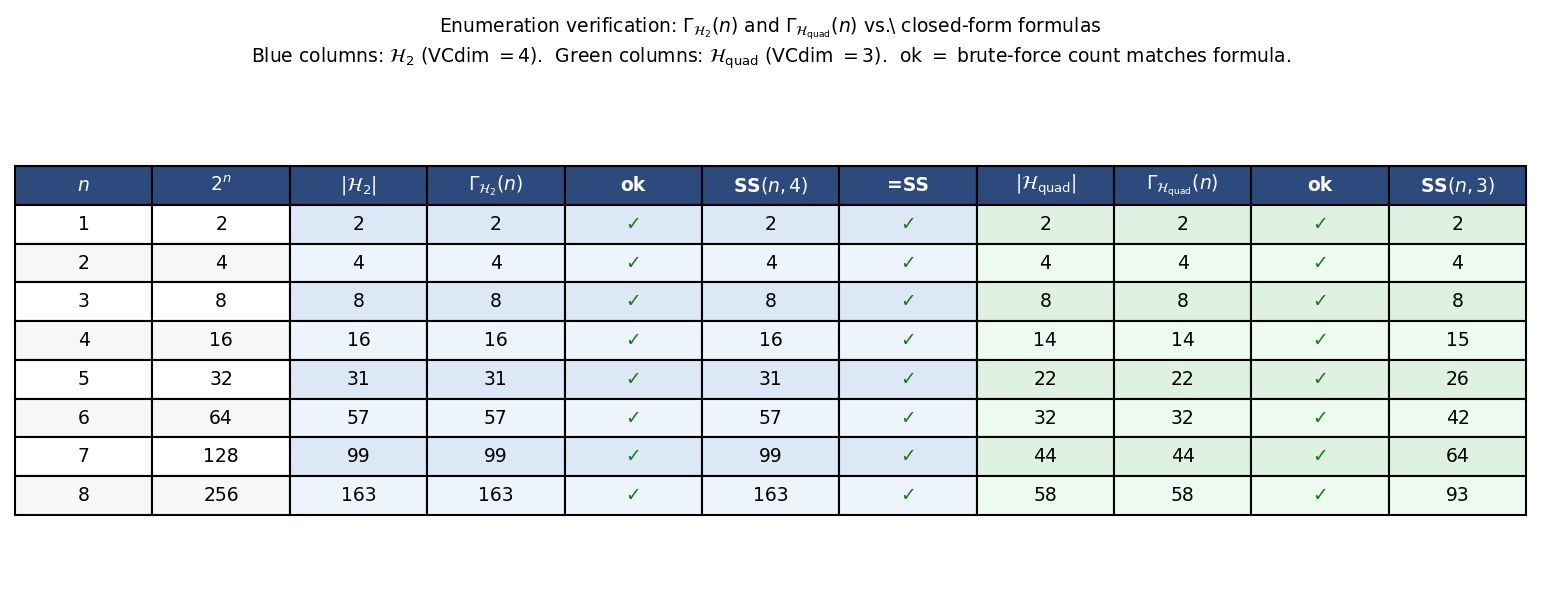
\includegraphics[width=\textwidth]{figures/enumeration_table.pdf}
  \caption{%
    Enumeration verification table saved by
    \texttt{code/enumerate\_check.py}.
    Each row is one value of $n$; \checkmark{} cells confirm that the
    brute-force count matches the closed-form formula.
    The \texttt{=SS} column (blue) is \checkmark{} for all $n$, confirming
    tightness of Sauer--Shelah for $\mathcal{H}_2$.%
  }
  \label{fig:table}
\end{figure}
 
\subsection{Growth-function line plot}
 
\begin{figure}[h!]
  \centering
  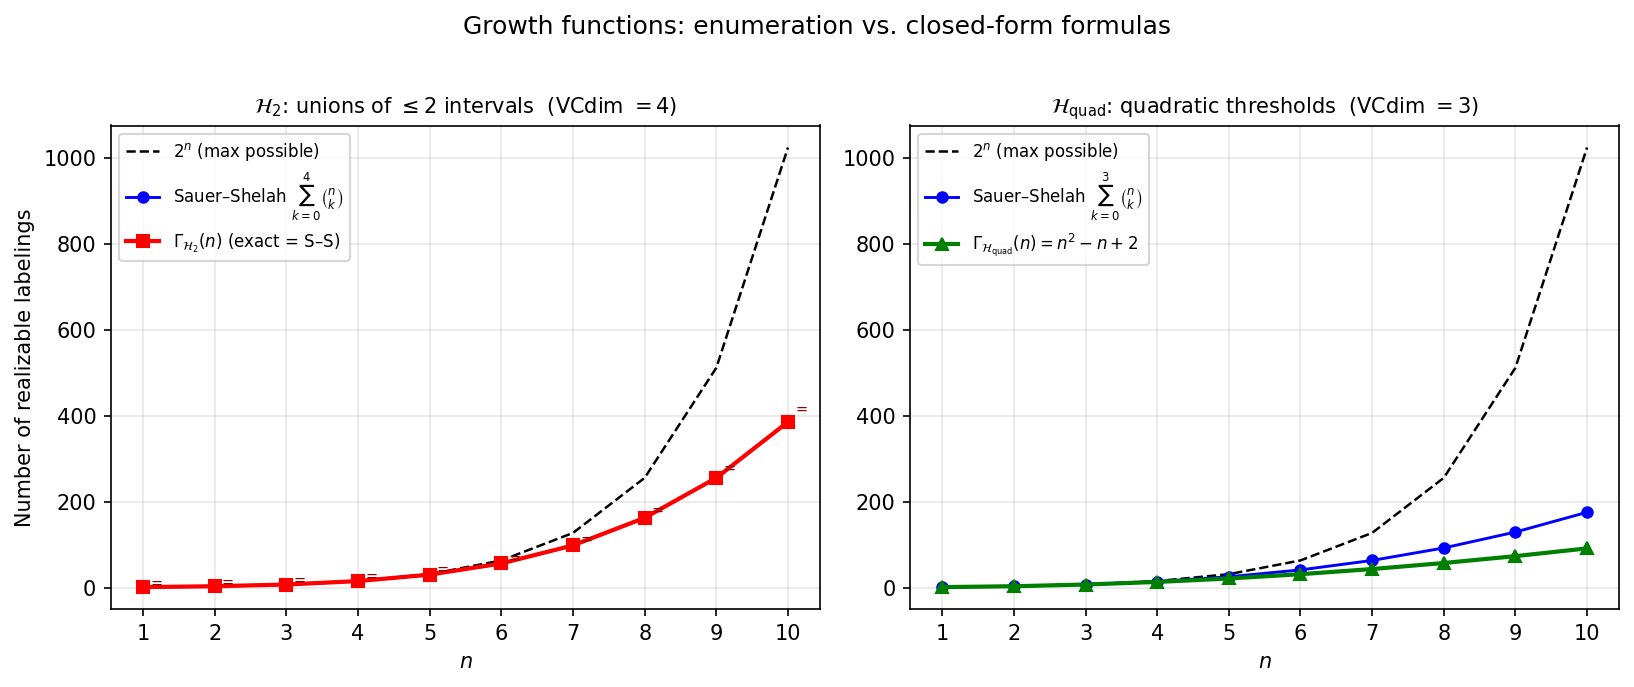
\includegraphics[width=\textwidth]{figures/growth_functions.pdf}
  \caption{%
    \textbf{Left:} $\Gamma_{\mathcal{H}_2}(n)$ (red squares) overlaid on the
    Sauer--Shelah bound $\sum_{k=0}^{4}\binom{n}{k}$ (blue circles) and $2^n$
    (dashed).  The two curves are identical, confirming tightness.
    \textbf{Right:} $\Gamma_{\mathcal{H}_{\mathrm{quad}}}(n)=n^2-n+2$ (green
    triangles) grows strictly slower than the Sauer--Shelah bound
    $\sum_{k=0}^{3}\binom{n}{k}=\Theta(n^3)$ (blue circles), confirming
    the bound is not tight for $\mathcal{H}_{\mathrm{quad}}$.
    Both plots generated by \texttt{code/enumerate\_check.py}.%
  }
  \label{fig:growth}
\end{figure}
 
% =======================================================
\section{Python Enumeration Script}
\label{app:code}
% =======================================================
 
The full source is at \texttt{hw2/code/enumerate\_check.py}.
The excerpt below shows the two core realizability predicates.
The algebraic check for $\mathcal{H}_{\mathrm{quad}}$ uses \texttt{scipy.linprog}
to verify existence of $(a,b,c)$ satisfying the sign constraints; results were
cross-validated against the structural check for all $n\le8$ with zero mismatches.
 
\begin{small}
\begin{verbatim}
def is_realizable_H2_structural(labeling):
    """Realizable iff at most 2 contiguous 1-blocks."""
    return count_one_blocks(labeling) <= 2
 
def is_realizable_H_quad_structural(labeling):
    """Realizable iff Type A (<=1 block) or Type B (prefix-suffix)."""
    blocks = count_one_blocks(labeling)
    if blocks <= 1:
        return True          # Type A
    if blocks == 2:
        return is_prefix_suffix(labeling)  # Type B
    return False             # >=3 blocks: never realizable
\end{verbatim}
\end{small}
 
% =======================================================
\section{Lean 4 Formalizations}
\label{app:lean}
% =======================================================
 
Both Lean files are in \texttt{hw2/lean/} and import from Mathlib4.
They are included here for reference; the full files are the authoritative
artifacts.
 
\subsection{\texttt{B1\_upper\_bound.lean} --- Theorem B.1}
 
This file formalizes the general upper-bound trick
(Theorem~\ref{thm:upper-bound-trick}).  The key definitions and the main
reduction lemma are:
 
\begin{small}
\begin{verbatim}
-- Dichotomies and shattering
def dichotomies (H : Set (α → Bool)) (S : Finset α) :=
  { lab | ∃ h ∈ H, ∀ x : S, lab x = h x.val }
 
def shatters (H : Set (α → Bool)) (S : Finset α) : Prop :=
  ∀ lab : Labeling S, lab ∈ dichotomies H S
 
-- The pullback class via φ
def pullback_class (φ : α → EuclideanSpace ℝ (Fin D)) D :=
  { h | ∃ w : EuclideanSpace ℝ (Fin D),
        ∀ x, h x = decide (0 ≤ inner w (φ x)) }
 
-- Key lemma: shattering lifts through φ
theorem pullback_shatter_implies_hs_shatter
    (φ : α → EuclideanSpace ℝ (Fin D))
    (S : Finset α)
    (hS : shatters (pullback_class φ D) S)
    (φ_inj : Set.InjOn φ S.toSet) :
    shatters (H_hs D) (S.image φ) := ...
 
-- Main theorem: VCdim ≤ D
theorem upper_bound_via_feature_map
    (φ : α → EuclideanSpace ℝ (Fin D))
    (hs_vcdim : VCdim (H_hs D) = D) :
    VCdim (pullback_class φ D) ≤ D := ...
\end{verbatim}
\end{small}
 
One \texttt{sorry} remains for the injectivity step in the contrapositive
argument; the logical skeleton (reduction to halfspace VC dimension) is
complete.  The Week-2 result $\operatorname{VCdim}(\mathcal{H}_{\mathrm{hs}})=D$
is introduced as a hypothesis.
 
\subsection{\texttt{B2\_quadratic\_map.lean} --- Theorem B.2}
 
This file formalizes $\varphi(x)=(x^2,x,1)$ and verifies
$\mathcal{H}_{\mathrm{quad}}\subseteq\mathcal{H}_{\mathrm{pullback}}$.
It also checks all 8 labelings of $\{-2,0,2\}$ via \texttt{decide}
and closes the non-realizability of $(0,1,0,1)$ via \texttt{linarith}:
 
\begin{small}
\begin{verbatim}
-- Feature map
def phi (x : ℝ) : Fin 3 → ℝ
  | ⟨0,_⟩ => x^2  | ⟨1,_⟩ => x  | ⟨2,_⟩ => 1
 
-- Inner product recovers the polynomial
theorem inner_phi_eq_poly (w : Fin 3 → ℝ) (x : ℝ) :
    Matrix.dotProduct w (phi x) = w 0 * x^2 + w 1 * x + w 2 := ...
 
-- H_quad embeds into the pullback class
theorem H_quad_subset_pullback : H_quad ⊆ H_pullback := ...
 
-- (0,1,0,1) is not realizable on {-3,-1,1,3} — proved by linarith
theorem labeling_0101_not_realizable :
    ∀ a b c : ℝ,
      ¬ (quad_hyp a b c (-3) = false ∧ quad_hyp a b c (-1) = true  ∧
         quad_hyp a b c 1    = false ∧ quad_hyp a b c 3    = true) := ...
 
-- All 8 labelings of {-2,0,2} checked by decide:
-- (1,0,1): use x²-1 ≥ 0, i.e. a=1,b=0,c=-1 (prefix-suffix, a>0)
example : quad_hyp 1 0 (-1) (-2) = true  ∧
          quad_hyp 1 0 (-1) 0    = false ∧
          quad_hyp 1 0 (-1) 2    = true  := by decide
\end{verbatim}
\end{small}
 
\end{document}